% Fig. 1 of the QRQT manuscript, standalone for Science Advances.
% Picture copied verbatim from _nc_work/floats/fig_qrqt.tex (lines 12-146); caption/label are in the main text.
\documentclass[border=2pt]{standalone}
% Minimal preamble shared by the two standalone QRQT figures (Science Advances build).
% Mirrors _sciadv_work/build_v2/nc_main.tex lines 29-62 (only what the pictures use).
\usepackage[T1]{fontenc}
\usepackage{amsmath}
\usepackage{newtxtext,newtxmath}   % Times-compatible, as in the AAAS science_template.tex
\usepackage{xcolor}
\usepackage{tikz}
\usetikzlibrary{calc,arrows.meta,positioning,backgrounds}
% colours used by the two TikZ figures (Fig. 1 and Fig. 4)
\definecolor{classwire}{RGB}{128,0,128}
\definecolor{boxgray}{RGB}{238,240,242}
\definecolor{textdark}{RGB}{48,54,60}
\definecolor{bellfill}{RGB}{220,231,223}
\definecolor{bellborder}{RGB}{122,145,130}
\definecolor{pqcfill}{RGB}{226,232,244}
\definecolor{pqcborder}{RGB}{96,118,156}
\definecolor{pqctext}{RGB}{78,100,138}
\definecolor{advcol}{RGB}{91,128,134}
\begin{document}
\begingroup % TikZ text at the sizes of the 10 pt APS layout the figure was drawn for
\renewcommand{\tiny}{\fontsize{5}{6}\selectfont}%
\renewcommand{\scriptsize}{\fontsize{7}{8}\selectfont}%
\renewcommand{\footnotesize}{\fontsize{8}{9.5}\selectfont}%
\renewcommand{\small}{\fontsize{9}{11}\selectfont}%
\renewcommand{\normalsize}{\fontsize{10}{12}\selectfont}%
\renewcommand{\large}{\fontsize{12}{14}\selectfont}%
\normalsize
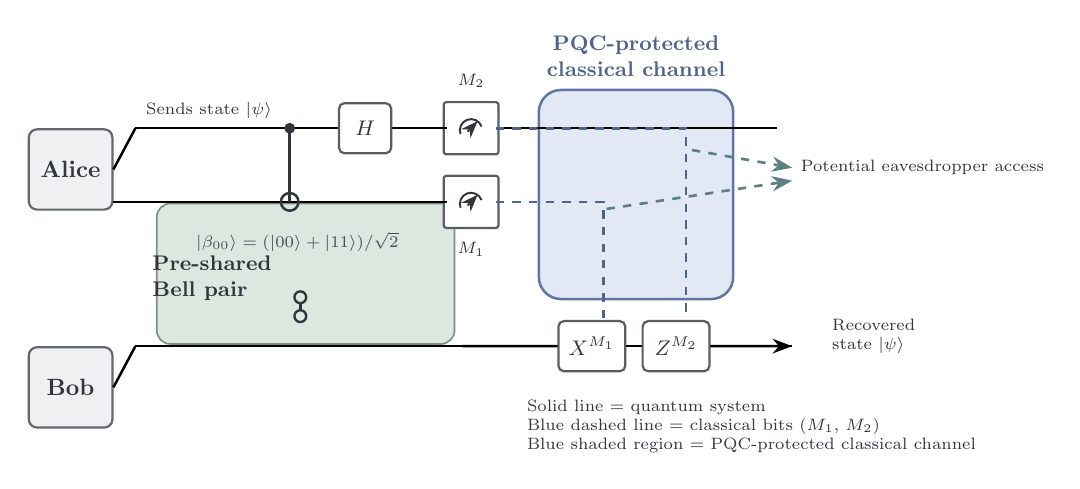
\begin{tikzpicture}[
    x=0.88cm,
    y=0.88cm,
    scale=0.85,
    transform shape,
    >=Stealth,
    thick,
    userbox/.style={
        draw=textdark!75,
        rounded corners=3pt,
        fill=boxgray,
        minimum width=1.25cm,
        minimum height=1.20cm,
        align=center
    },
    gate/.style={
        draw=textdark!80,
        rounded corners=2pt,
        minimum width=0.90cm,
        minimum height=0.75cm,
        fill=white,
        inner sep=1.2pt
    },
    meas/.style={
        draw=textdark!80,
        rounded corners=1pt,
        minimum width=0.82cm,
        minimum height=0.78cm,
        fill=white
    },
    classpath/.style={
        draw=pqctext,
        dashed,
        line width=0.95pt,
        ->,
        >=Stealth
    },
    advpath/.style={
        draw=advcol,
        dashed,
        line width=0.95pt,
        ->,
        >=Stealth
    }
]
%
\node[userbox, text=textdark, font=\bfseries\normalsize] (alice) at (0,1.75) {Alice};
\node[userbox, text=textdark, font=\bfseries\normalsize] (bob)   at (0,-1.95) {Bob};
%
\draw[black, line width=0.9pt] (1.10,2.45) -- (12.00,2.45);
\draw[black, line width=0.9pt] (1.10,1.20) -- (6.00,1.20);
\draw[black, line width=0.9pt] (1.10,-1.25) -- (12.25,-1.25);
%
\node[above, text=textdark, font=\scriptsize] at (2.35,2.47) {Sends state $|\psi\rangle$};
%
\draw[black, line width=0.9pt] (alice.east) -- (1.10,2.45);
\draw[black, line width=0.9pt] (alice.east |- 1.10,1.20) -- (1.10,1.20);
\draw[black, line width=0.9pt] (bob.east) -- (1.10,-1.25);
%
\begin{scope}[on background layer]
\node[
    rectangle,
    rounded corners=5pt,
    fill=bellfill,
    draw=bellborder,
    line width=0.6pt,
    minimum width=4.45cm,
    minimum height=2.10cm,
    anchor=west,
    inner sep=0pt
] (bell) at (1.45,-0.02) {};
\end{scope}
%
\node[align=left, text=textdark, font=\bfseries\small] at (2.40,-0.10) {Pre-shared\\Bell pair};
\node[text=textdark!90, font=\scriptsize] at (3.85,0.52) {$|\beta_{00}\rangle=(|00\rangle+|11\rangle)/\sqrt{2}$};
%
\draw[line width=0.85pt, draw=textdark] (3.90,-0.42) circle (0.10);
\draw[line width=0.85pt, draw=textdark] (3.90,-0.74) circle (0.10);
\draw[line width=0.95pt, draw=textdark] (3.90,-0.52) -- (3.90,-0.64);
%
\node[gate, minimum width=0.78cm, text=textdark, font=\small] (H) at (5.00,2.45) {$H$};
%
\filldraw[textdark] (3.72,2.45) circle (1.8pt);
\draw[textdark, line width=0.9pt] (3.72,2.45) -- (3.72,1.20);
\draw[textdark, line width=0.9pt] (3.72,1.20) circle (0.15);
%
\node[meas] (M2box) at (6.80,2.45) {};
\node[meas] (M1box) at (6.80,1.20) {};
%
\draw[line width=0.7pt, draw=textdark] (6.62,2.35) arc[start angle=200,end angle=20,radius=0.19];
\draw[->, line width=0.7pt, draw=textdark] (6.74,2.39) -- (6.91,2.57);
%
\draw[line width=0.7pt, draw=textdark] (6.62,1.10) arc[start angle=200,end angle=20,radius=0.19];
\draw[->, line width=0.7pt, draw=textdark] (6.74,1.14) -- (6.91,1.32);
%
\node[above=2pt, text=textdark, font=\scriptsize] at (M2box.north) {$M_2$};
\node[below=2pt, text=textdark, font=\scriptsize] at (M1box.south) {$M_1$};
%
\draw[black, line width=0.9pt] (5.65,2.45) -- (6.39,2.45);
\draw[black, line width=0.9pt] (5.65,1.20) -- (6.39,1.20);
%
\begin{scope}[on background layer]
\path[
    fill=pqcfill,
    draw=pqcborder,
    line width=0.9pt,
    rounded corners=8pt
] (7.95,3.10) rectangle (11.25,-0.45);
\end{scope}
%
\node[align=center, text=pqctext, font=\bfseries\small] at (9.60,3.68) {PQC-protected\\classical channel};
%
\draw[classpath] (7.22,2.45) -- (10.45,2.45) -- (10.45,-1.25);
\draw[classpath] (7.22,1.20) -- (9.05,1.20) -- (9.05,-1.25);
%
\node[gate, minimum width=1.00cm, text=textdark, font=\small] (Xcorr) at (8.85,-1.25) {$X^{M_1}$};
\node[gate, minimum width=1.00cm, text=textdark, font=\small] (Zcorr) at (10.28,-1.25) {$Z^{M_2}$};
%
\draw[black, line width=0.9pt] (6.65,-1.25) -- (Xcorr.west);
\draw[black, line width=0.9pt] (Xcorr.east) -- (Zcorr.west);
\draw[->, black, line width=0.9pt] (Zcorr.east) -- (12.25,-1.25);
%
\node[align=left, anchor=west, text=textdark, font=\scriptsize] at (12.78,-1.08) {Recovered\\state $|\psi\rangle$};
%
\node[right, text=textdark, font=\scriptsize] (advtext) at (12.25,1.78) {Potential eavesdropper access};
\draw[advpath] (10.55,2.08) -- (12.25,1.78);
\draw[advpath] (9.10,1.08) -- (12.25,1.56);
%
\node[align=left, anchor=north west, text=textdark, font=\scriptsize] at (7.60,-2.02) {
Solid line = quantum system\\
Blue dashed line = classical bits ($M_1$, $M_2$)\\
Blue shaded region = PQC-protected classical channel
};
%
\end{tikzpicture}
\endgroup
\end{document}
